\par\vspace{1em}
\begin{longtable}{|c|c|c|}
  \hline
  \rule[-0.5em]{0pt}{1.8em} & \rule[-0.5em]{0pt}{1.8em} $G$ & \rule[-0.5em]{0pt}{1.8em} $G'$ \\
  \hline
  \endhead
  \hline
  \endfoot
  \caption{Ejemplos de contenencia de grafos} \addtocounter{table}{-1}\refstepcounter{table}\label{tab:grafos} \\
  \endlastfoot

  $G_1 \subseteq G'_1$ &
  \begin{minipage}{0.3\textwidth} \centering \vspace{8pt} \resizebox{0.85\linewidth}{!}{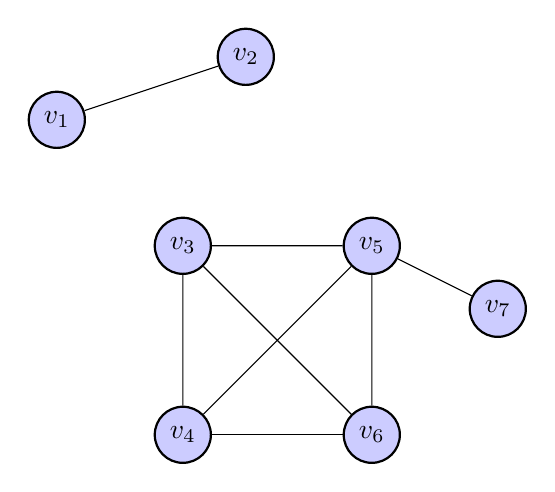
\begin{tikzpicture}
   [scale=.8,auto=left,every node/.style={circle,fill=blue!20,draw=black,thick}]
  \node (n1) at (0,5) {$v_1$};
  \node (n2) at (3,6) {$v_2$};
  \node (n3) at (2,3) {$v_3$};
  \node (n4) at (2,0) {$v_4$};
  \node (n5) at (5,3) {$v_5$};
  \node (n6) at (5,0) {$v_6$};
  \node (n7) at (7,2) {$v_7$};

  \foreach \from/\to in {n1/n2, n3/n5, n5/n6, n6/n4, n4/n3, n3/n6, n4/n5, n5/n7}
    \draw (\from) -- (\to);

\end{tikzpicture}
} \vspace{6pt} \end{minipage} &
  \begin{minipage}{0.3\textwidth} \centering \vspace{8pt} \resizebox{0.85\linewidth}{!}{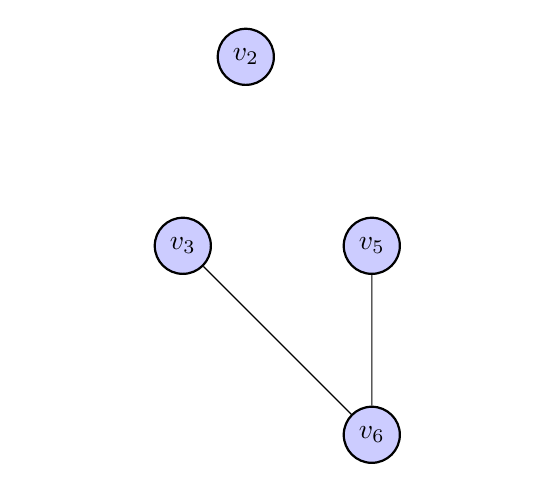
\begin{tikzpicture}
  [scale=.8,auto=left,every node/.style={circle,fill=blue!20,draw=black,thick}]
  \node (n1) at (0,5) [opacity=0] {$v_1$};
  \node (n2) at (3,6) {$v_2$};
  \node (n3) at (2,3) {$v_3$};
  \node (n4) at (2,0) [opacity=0]{$v_4$};
  \node (n5) at (5,3) {$v_5$};
  \node (n6) at (5,0) {$v_6$};
  \node (n7) at (7,2) [opacity=0]{$v_7$};

  \foreach \from/\to in {n1/n2, n3/n5, n5/n6, n6/n4, n4/n3, n3/n6, n4/n5, n5/n7}
    \draw[opacity=0] (\from) -- (\to);
   
    \foreach \from/\to in {n3/n6, n5/n6}
     \draw[opacity=1] (\from) -- (\to);

  \end{tikzpicture}
} \vspace{6pt} \end{minipage} \\
  \hline

  $G_2 \subseteq G'_2$ &
  \begin{minipage}{0.3\textwidth} \centering \vspace{8pt} \resizebox{0.8\linewidth}{!}{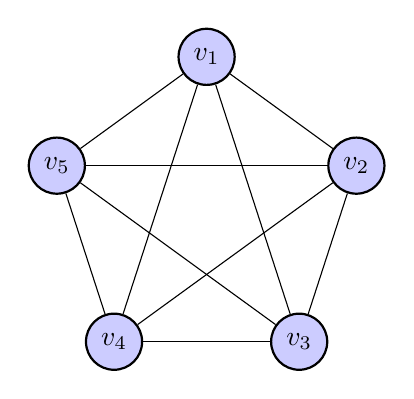
\begin{tikzpicture}
  [scale=1,auto=left,every node/.style={circle,fill=blue!20,draw=black,thick}]
  \node (n1) at (90:2) {$v_1$};
  \node (n2) at (18:2) {$v_2$};
  \node (n3) at (-54:2) {$v_3$};
  \node (n4) at (-126:2) {$v_4$};
  \node (n5) at (-198:2) {$v_5$};

  \foreach \from/\to in {n1/n2, n1/n3, n1/n4, n1/n5, n2/n3, n2/n4, n2/n5, n3/n4, n3/n5, n4/n5}
    \draw (\from) -- (\to);

 \end{tikzpicture}
} \vspace{6pt} \end{minipage} &
  \begin{minipage}{0.3\textwidth} \centering \vspace{8pt} \resizebox{0.8\linewidth}{!}{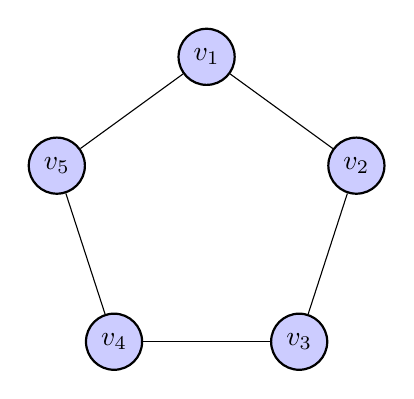
\begin{tikzpicture}
  [scale=1,auto=left,every node/.style={circle,fill=blue!20,draw=black,thick}]
  \node (n1) at (90:2) {$v_1$};
  \node (n2) at (18:2) {$v_2$};
  \node (n3) at (-54:2) {$v_3$};
  \node (n4) at (-126:2) {$v_4$};
  \node (n5) at (-198:2) {$v_5$};

  \foreach \from/\to in {n1/n2, n2/n3, n3/n4, n4/n5, n5/n1}
    \draw (\from) -- (\to);

 \end{tikzpicture}
} \vspace{6pt} \end{minipage} \\
  \hline

  $G_3 \subseteq G'_3$ &
  \begin{minipage}{0.3\textwidth} \centering \vspace{8pt} \resizebox{0.8\linewidth}{!}{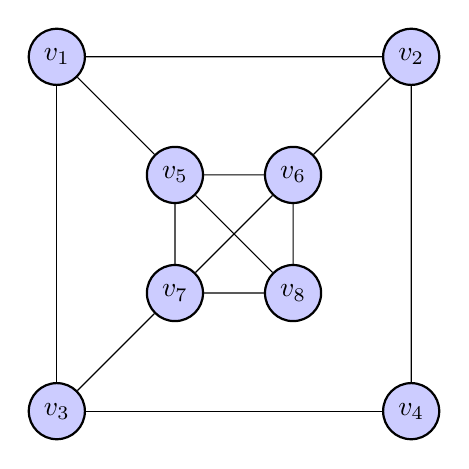
\begin{tikzpicture}
  [scale=1.5,auto=left,every node/.style={circle,fill=blue!20,draw=black,thick}]
  \node (n1) at (0,3) {$v_1$};
  \node (n2) at (3,3) {$v_2$};
  \node (n3) at (0,0) {$v_3$};
  \node (n4) at (3,0) {$v_4$};
  \node (n5) at (1,2) {$v_5$};
  \node (n6) at (2,2) {$v_6$};
  \node (n7) at (1,1) {$v_7$};
  \node (n8) at (2,1) {$v_8$};

  \foreach \from/\to in {n1/n2, n1/n3, n2/n4, n3/n7, n6/n7, n1/n5, n2/n6, n5/n6, n6/n8, n7/n8, n7/n5, n5/n8, n3/n4}
    \draw (\from) -- (\to);

 \end{tikzpicture}
} \vspace{6pt} \end{minipage} &
  \begin{minipage}{0.3\textwidth} \centering \vspace{8pt} \resizebox{0.8\linewidth}{!}{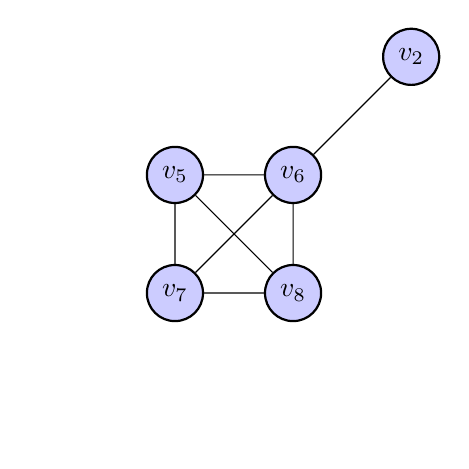
\begin{tikzpicture}
  [scale=1.5,auto=left,every node/.style={circle,fill=blue!20,draw=black,thick}]
  \node (n1) at (0,3) [opacity=0] {$v_1$};
  \node (n2) at (3,3) {$v_2$};
  \node (n3) at (0,0) [opacity=0] {$v_3$};
  \node (n4) at (3,0) [opacity=0] {$v_4$};
  \node (n5) at (1,2) {$v_5$};
  \node (n6) at (2,2) {$v_6$};
  \node (n7) at (1,1) {$v_7$};
  \node (n8) at (2,1) {$v_8$};

  \foreach \from/\to in {n2/n6, n5/n6, n6/n8, n7/n8, n7/n5, n5/n8, n6/n7}
    \draw (\from) -- (\to);

 \end{tikzpicture}
} \vspace{6pt} \end{minipage} \\
  \hline
\end{longtable}
\par\vspace{-0.3em}
